
\begin{figure*}[ht!]
  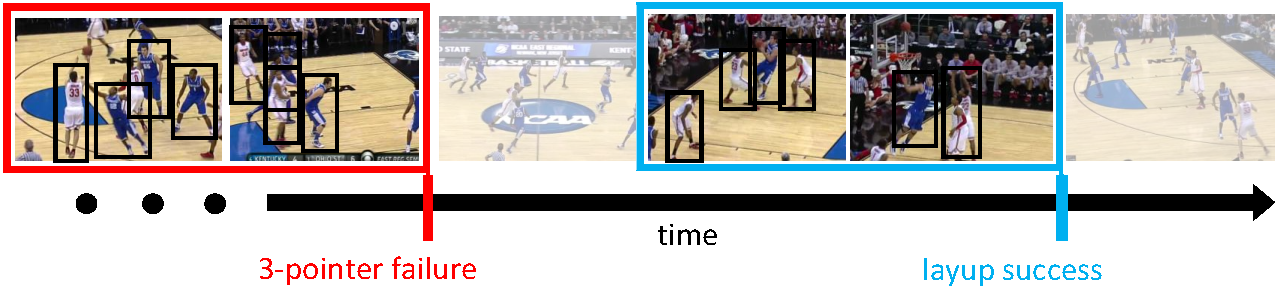
\includegraphics[width=7 in]{images/dataset_figure_cropped.pdf}
  \caption{Our dataset contains timestamp annotations for 11 basketball events
    in long untrimmed videos. Additionally, we also provide bounding boxes for player
    detections obtained from a multibox model trained on a subset of training
  video frames.}
\end{figure*}

\section{NCAA Basketball Dataset}

Most recent activity detection datasets like THUMOS \cite{THUMOS},
ActivityNet \cite{ActivityNet}, UCF101 
\cite{UCF101}, finegrained cooking \cite{Finegrained_cooking},
mostly contain videos with a single actor performing one activity.
By contrast, we are interested in settings where there are multiple
people in each frame, only a small number of whom are involved with
the  activity. In such setting, we are interested in recognizing the event
as well as the key participants. A natural choice for such data is
multi-player team sports.

In this paper, we focus on basketball games, although our techniques
are general purpose.
In particular,  we use a subset of the $296$ NCAA games available from 
YouTube\footnote{https://www.youtube.com/user/ncaaondemand}.  These games are
played in different venues over different periods of time.
We only consider the most recent $257$ games, since older games used
slightly different rules than modern basketball.

\begin{table}[ht!]
\begin{center}
\small
 \begin{tabular}{|l|c|c|}
  \hline
  Event          & \# Videos Train (Test) & Avg. \# people \\ \hline \hline
  3-point succ.    & 895 (188) &  8.35 \\ 
  3-point fail.    & 1934 (401) &  8.42 \\ 
  free-throw succ. & 552 (94) &  7.21\\ 
  free-throw fail. & 344 (41) &  7.85\\  
  layup succ.      & 1212 (233) &  6.89\\ 
  layup fail.      & 1286 (254) &  6.97 \\ 
  2-point succ.    & 1039 (148) &  7.74 \\ 
  2-point fail.    & 2014 (421) &  7.97\\ 
  slam dunk succ.  & 286 (54) &  6.59 \\ 
  slam dunk fail.  & 47 (5) &  6.35\\ 
  steal & 1827 (417) & 7.05\\ \hline  
  \end{tabular}
\end{center}
  \caption{The number of videos per event in our dataset along with
  the average number of people per video corresponding to each of the
events. The number of people is higher than existing datasets for
multi-person event recognition.}
  \label{tab:data_dist}
\end{table}

The NCAA dataset is accompanied by freeform play-by-play text snippets
describing the events at a few key-moments in each game.  Unfortunately, the
temporal frequency of this annotation is too sparse to be useful for training /
testing an event detection system.  So we decided to use Amazon Mechanical Turk
(AMT) to annote the events in these videos. We will release our annotated data
upon paper acceptance.

To determine the set of events, we clustered the play-by-play text to identify
the most frequent events from all games. We narrowed the event list to $11$
classes, listed in Tab.~\ref{tab:data_dist}.  In particular, we considered
5 types of shots, each of which could be succesful or failed, plus a steal
event. 

We setup an AMT task, where the annotators were asked to annotate the
``end-point" of these events if and when they occur in the videos.  To
determine the starting time, we assumed that each event was 4 seconds long.
The complete game videos are typically $1.5$ hours long.

The videos were randomly split into $212$ training, $12$ validation and $33$
test videos.  We split each of these videos into 4 second clips (using the
annotation boundaries), and subsampled these to 6fps.  We filter out clips
which are not profile shots (such as those shown in Figure~\ref{fig:model})
using a separately trained classifier; this excludes close up shots of players,
animations, as well as crowd shots.  This resulted in a total of $11436$
training, $856$ validation and $2256$ test clips, each of which has one of 11
labels.

Note that our dataset is comparable in size to the THUMOS'15 detection
challenge ($XXXX$ trimmed training instances for $20$ classes and $6553$
untrimmed validation instances). The distribution of annotations across all the
different events is visualized in Fig.~\ref{fig:data_dist}, with sample videos
for a few event classes. To the best of our
knowledge, this is the first dataset with dense temporal annotations for
such long video sequences.

\noindent \textbf{Player detections}
We also used AMT to annotate the bounding boxes of all the players in a
subset \KEVIN{HOW BIG?} of frames from the training videos.
We then trained a Multibox detector \cite{Szegedy_arxiv14}
with these annotatoins, and ran the trained detector on all the videos in our dataset.
We retained all detections above a confidence of 0.5 per frame;
this resulted in person detections as listed in Tab.~\ref{tab:table_stats}.
The multibox model achieves an average overlap of $0.7$ at a recall of $0.8$
with ground-truth bounding boxes in the validation videos.
 \TODO{Get exact numbers from John.}
These detected player bounding boxes from the
multi-box model will also be made available with the dataset.
